\chapter{Introduction}
This chapter provides the common thread of the work and positions it within the broader field of robotic manipulation and human-robot collaboration. 
We first develop the \emph{motivation} for the study, followed by a precise \emph{problem description}, a formal \emph{problem statement}, and the resulting \emph{aim of the work}. 
Subsequent chapters present the State of the Art, the proposed methods, the experimental evaluation, a discussion of the results and their implications, and an outlook on future research directions.

    \section{Motivation}
    The motivation for this work is given in two subsections, where the \emph{Context} subsection outlines the growing role of industrial and collaborative manipulators,
    while the \emph{Use Case} subsection specifies a concrete manipulation scenario that requires accurate online identification of robot and payload parameters.

        \subsection{Context}
        As the robotics industry grows year over year, so does the number of robots operating around the world. It is estimated that there were approximately 3.4 million industrial robots in use worldwide in
        2023~\cite{Q0_1_industrial_robots_in_operation}. At the same time, the number of newly installed industrial robots has been increasing steadily since 2014; between 2021 and 2024, around 541\,000 new industrial
        robots were installed per year~\cite{Q0_2_industrial_robots_new_installations}. Within this landscape, collaborative robots (cobots) represent about 10.5\% of the industrial robot market, with 57\,040 new units 
        deployed in 2023, and annual cobot installations since 2020, 2022, and 2023 reaching roughly 50\,000 units per year; importantly, these cobots are expected to complement rather than replace traditional industrial 
        robots~\cite{Q0_3_industrial_robots_new_cobot_installations_BarChart}.

        \begin{figure}[ht]
            \centering
            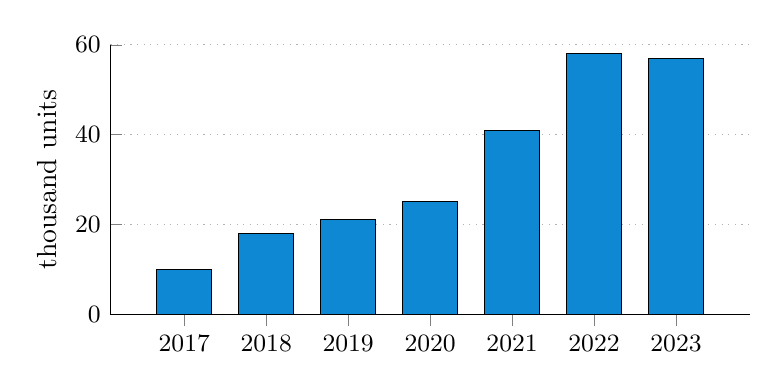
\begin{tikzpicture}
                \begin{axis}[
                        ybar,
                        bar width=20pt,
                        ymin=0, ymax=60,
                        width=0.8\linewidth,
                        height=5cm,
                        enlarge x limits=0.15,
                        axis x line*=bottom,
                        axis y line*=left,
                        ymajorgrids=true,
                        grid style={dotted,gray!60},
                        ylabel={thousand units},
                        xtick=data,
                        xticklabels={2017,2018,2019,2020,2021,2022,2023},
                        tick label style={font=\small},
                    ]
                    \addplot[fill=cyan!70!blue] coordinates {
                            (1,10)  % 2017
                            (2,18)  % 2018
                            (3,21)  % 2019
                            (4,25)  % 2020
                            (5,41)  % 2021
                            (6,58)  % 2022
                            (7,57)  % 2023
                        };
                \end{axis}
            \end{tikzpicture}
            \caption{Global annual installations of collaborative robots from 2017 to 2023 (in thousand units). Data from~\cite{Q0_3_industrial_robots_new_cobot_installations_BarChart}.}\label{fig:cobot_installations}
        \end{figure}

        The growing deployment of, and increasing collaboration with, robots imposes stringent requirements on safety and performance. 
        As tasks become more complex and humans and robots share workspaces more closely, two closely related problems become central: 
        safe manipulation of payloads and safe physical human-robot interaction. 
        Addressing both problems requires accurate knowledge of the inertial parameters of the manipulated object together with consistent estimation of the robot's dynamic state and interaction forces. 
        A collaborative robot must therefore maintain an internal representation of the mass-inertia properties of the payload or tool it manipulates and of the forces exchanged with its environment. 
        This dynamic awareness is a prerequisite for compliant, contact-rich behaviour and for precise, high-performance manipulation in close proximity to humans.
        \cite{Q1_1_fast_inertial_id_cobots, Q1_2_online_payload_mo, Q1_3_external_torque_smo, Q1_5_payload_estimation_compensation_2025, Q1_7_10947736, Q1_8_10944553, Q1_9_xu2022_double_weighting_payload_id, % chktex 2
        Q1_10_duan_payload_ftsensor, Q1_11_wei_composite_filter, Q1_13_dynamic_model_id_swevers2007, Q1_14_long2022sliding_momentum_observer, Q3_2_encoder_attention_payload}.

        \subsection{Use Case}

        The considerations above motivate a concrete use case in which a collaborative robotic arm must manipulate previously unseen objects in a shared workspace. 
        A vision system can provide geometric information such as shape and dimensions of the payload, but it does not directly reveal its mass, center of mass (CoM), or inertia tensor. 
        For safe and precise execution of contact-rich tasks, however, these inertial properties are indispensable.

        In practice, the only viable way to obtain this information during operation is to exploit the robot's own sensor data, such as joint positions, velocities and accelerations, motor currents/torques,
        and optionally wrist force/torque measurements. 
        From these signals, one can estimate both the robot's rigid-body parameters and the inertial properties of the attached payload. 
        This leads to the dual identification problem of \emph{robot dynamic parameter identification} (RDPI) and \emph{payload dynamic parameter identification} (PDPI).

        The targeted application scenario comprises typical industrial and collaborative tasks such as pick-and-place, human-assisted manipulation, and precise tool use. 
        In all these cases, RDPI and PDPI must be performed online so that the controller maintains an up-to-date model of the combined robot-payload dynamics and the resulting contact forces. 
        Robust online identification methods are therefore a key enabling technology for safe human-robot collaboration and high-performance manipulation with arbitrary payloads and tools.

    \section{Problem Statement}
    The subsection \emph{Kinematic and Dynamic Background of Robot Manipulation} analyses why endowing a robotic manipulator with awareness of its own dynamics, payload, and tools is mathematically demanding and cannot be
    achieved by simple calculation or direct measurement alone. The subsection \emph{Limitations of the Current State of the Art} then identifies the main shortcomings of existing identification and estimation methods
    in the literature, thereby motivating the contribution of this work.

        \subsection{Kinematic and Dynamic Background of Robot Manipulation}
        \label{sec:robot_dynamics_background}
        The inertial properties of a rigid body are collected in the standard 10-dimensional parameter vector
        \begin{equation}
        \boldsymbol{\phi}^T
        =
        \begin{bmatrix}
            m & m c_x & m c_y & m c_z &
            J_{xx} & J_{xy} & J_{xz} & J_{yy} & J_{yz} & J_{zz}
        \end{bmatrix}
        \in \mathbb{R}^{10},
        \label{eq:rigidBody}
        \end{equation}
        which enters the Newton-Euler equations
        \begin{equation}
        \begin{bmatrix} 
            \mathbf{f} \\[2pt] \boldsymbol{\tau}
        \end{bmatrix}
        =
        m
        \begin{bmatrix}
            \mathbf{I}_{3\times3} & -[\mathbf{c}]^{\times} \\
            [\mathbf{c}]^{\times} & \mathbf{J}_s
        \end{bmatrix}
        \begin{bmatrix}
            \mathbf{a} \\[2pt] \boldsymbol{\alpha}
        \end{bmatrix}
        +
        \begin{bmatrix}
            m[\boldsymbol{\omega}]^{\times}[\boldsymbol{\omega}]^{\times}\mathbf{c} \\
            [\boldsymbol{\omega}]^{\times}\mathbf{J}_s\boldsymbol{\omega}
        \end{bmatrix},
        \label{eq:newtonEuler}
        \end{equation}
        so that the wrench $(\mathbf{f},\boldsymbol{\tau})$ depends nonlinearly on the motion $(\mathbf{a},\boldsymbol{\alpha},\boldsymbol{\omega})$ but linearly on $\boldsymbol{\phi}$.
        
        For the equipment rigidly attached to the tool flange (gripper/tool, with or without payload/load) we define an effective rigid-body parameter vector
        \begin{equation}
        \boldsymbol{\phi}_{\mathrm{eff}}
        =
        \begin{cases}
            \boldsymbol{\phi}_{\mathrm{tool}}, & \text{no load},\\[4pt]
            \boldsymbol{\phi}_{\mathrm{tool}} + \boldsymbol{\phi}_{\mathrm{load}}, & \text{with load},
        \end{cases}
        \label{eq:rigidEffective}
        \end{equation}
        which acts on top of the nominal robot dynamics. In contrast, with a clean flange (no tool/no load) only the robot parameters $\boldsymbol{\phi}_{\mathrm{robot}}$ contribute to the system dynamics.


        The robot structure itself is described by its own parameter vector $\boldsymbol{\phi}_{\mathrm{robot}}$, which enters the standard joint-space rigid-body dynamics. We denote this contribution by
        $\boldsymbol{\tau}_{\mathrm{robot}}$ (clean flange),
        \begin{equation}
        \boldsymbol{\tau}_{\mathrm{robot}}
        =
        \mathbf{M}(\mathbf{q}) \ddot{\mathbf{q}}
        +
        \mathbf{C}(\mathbf{q},\dot{\mathbf{q}})\dot{\mathbf{q}}
        +
        \mathbf{G}(\mathbf{q})
        +
        \boldsymbol{\tau}_f(\dot{\mathbf{q}}),
        \label{eq:robot_dynamics}
        \end{equation}
        where $\boldsymbol{\tau}_f(\dot{\mathbf{q}})$ models joint-level non-idealities such as Coulomb and viscous friction,
        possible Stribeck effects, and drive-train phenomena like backlash.
        
        The wrench generated by the effective rigid body at the flange induces an additional joint-space torque
        \begin{equation}
        \boldsymbol{\tau}_{\mathrm{ext}}
        =
        \mathbf{J}^T(\mathbf{q})\,\vec{F}_{\mathrm{ext}}(\boldsymbol{\phi}_{\mathrm{eff}}),
        \label{eq:tau_ext}
        \end{equation}
        where $\mathbf{J}(\mathbf{q})$ is the end-effector Jacobian. In the clean-flange case (no tool/no load), $\vec{F}_{\mathrm{ext}}$ reduces to purely external interaction forces with the environment (e.g.\ contacts or collisions).

    

        The motor torques are therefore
        \begin{equation}
        \boldsymbol{\tau}_{\mathrm{motor}}
        =
        \boldsymbol{\tau}_{\mathrm{robot}}
        +
        \boldsymbol{\tau}_{\mathrm{ext}}(\boldsymbol{\phi}_{\mathrm{eff}}),
        \label{eq:tau_motor}
        \end{equation}
        and for brushless DC actuators with torque constant $k_t$ one obtains the current–torque relation
        \begin{equation}
        \boldsymbol{\tau}_{\mathrm{motor}} = k_t\,\boldsymbol{I}
        \quad\Rightarrow\quad
        \boldsymbol{I}
        =
        \frac{\boldsymbol{\tau}_{\mathrm{robot}}
                + \boldsymbol{\tau}_{\mathrm{ext}}(\boldsymbol{\phi}_{\mathrm{eff}})}
            {k_t}.
        \label{eq:I_payload}
        \end{equation}

        If a force/torque sensor is mounted at the flange, the measured wrench can be written, using the relations derived in the Appendix, as
        \begin{equation}
        \vec{F}_{\mathrm{measured}}
        =
        Y\bigl(\mathbf{a},\boldsymbol{\alpha},\boldsymbol{\omega}\bigr)\,
        \boldsymbol{\phi}_{\mathrm{eff}}
        +
        \vec{F}_{\mathrm{bias}}
        +
        \vec{n},
        \label{eq:F_measured_regressor}
        \end{equation}

        where $Y(\cdot)$ is the $6\times 10$ Newton-Euler regressor matrix defined in the Appendix \ref{app:query_categories}. It is linear in the inertial parameter vector $\boldsymbol{\phi}_{\mathrm{eff}}$, but depends nonlinearly on the motion variables $(\mathbf{a},\boldsymbol{\alpha},\boldsymbol{\omega})$. The terms $\vec{F}_{\mathrm{bias}}$ and $\vec{n}$ denote sensor bias and noise, respectively.\footnote{All experiments in this work are simulation-based; in the subsequent method formulation, sensor bias and noise are therefore neglected and \eqref{eq:F_measured_regressor} is used without $\vec{F}_{\mathrm{bias}}$ and $\vec{n}$.}
        The motion variables $(\mathbf{a},\boldsymbol{\alpha},\boldsymbol{\omega})$ are in turn determined by the joint state and motor torques through the nonlinear dynamics
        \eqref{eq:robot_dynamics}--\eqref{eq:I_payload}.

        From an identification viewpoint, this creates two tightly coupled challenges. 
        First, all available measurements (joint currents, positions, velocities and flange wrench) depend on the \emph{combined} dynamics of robot, tool and load via the nonlinear relationships~\eqref{eq:robot_dynamics}-\eqref{eq:F_measured_regressor}, so the contribution of the load parameters $\boldsymbol{\phi}_{\mathrm{load}}$ cannot be isolated by simple computation or direct measurement. 
        Second, accurate payload or load dynamic parameter identification (PDPI) presupposes an equally accurate compensation of the underlying robot–tool dynamics, including unmodelled effects such as friction and joint transmission nonlinearities. 
        Together, these aspects make dynamic awareness of payload, tool and robot a mathematically demanding inverse problem rather than a straightforward calculation from geometric or sensor data.

        \subsection{Limitations of the Current State of the Art}

        The SoA analysis in reveals several recurring gaps that are directly relevant for this work:

        \begin{itemize}
        \item \textbf{Weak and fragmentary treatment of payload inertia and effective rigid body.}
        In Q1, payload mass (and often CoM) can be estimated accurately, but inertia tensors are frequently weakly excited, ill-conditioned or only partially validated, especially in cobot-safe regimes~\cite{Q1_1_fast_inertial_id_cobots,Q1_5_payload_estimation_compensation_2025,Q1_7_10947736,Q1_10_duan_payload_ftsensor,Q1_16_xu_payload_difference_2024} %\cite{Q1_1, Q1_5, Q1_7, Q1_10, Q1_16}
        Q2-Q4 largely \emph{assume} fixed tools/payloads and do not identify the full effective rigid body at all~\cite{Q2_1_contact_force_gp_observer,Q2_4_GIACOMUZZO20231584,Q3_3_lstm_force_estimation,Q3_4_asgrnn_force_observer,Q4_1_extended_delan_motor,Q4_3_residual_pinns_dynamics_id,Q4_4_10729277} %\cite{Q2_1, Q2_4, Q3_3, Q3_4, Q4_1, Q4_3, Q4_4}
        As a result, there is no robust, general mechanism to obtain and maintain an accurate $\boldsymbol{\phi}_{\mathrm{eff}}$ that could be used systematically for tool/gripper compensation and subsequent PDPI.

        \item \textbf{Entangled or black-box treatment of friction, transmission and contact effects.}
        Many observer-based and LS/NE methods in Q1 are highly sensitive to imperfect friction and transmission models; errors grow around velocity reversals and at higher speeds, even with advanced observers or NN friction terms~\cite{Q1_3_external_torque_smo,Q1_4_contact_force_kf,Q1_6_hu2025_fdrdi,Q1_12_han_finite_time_observer,Q1_15_tang2023wls_rwspo,Q1_17_liu2021sensorless_dob_nn} %\cite{Q1_3, Q1_4, Q1_6, Q1_12, Q1_15, Q1_17}
        Q2 explicitly models all unmodelled dynamics, friction and contacts as a single GP disturbance~\cite{Q2_1_contact_force_gp_observer,Q2_2_contact_force_gpadkf,Q2_3_contact_detection_gp}, %\cite{Q2_1, Q2_2, Q2_3}
        which improves prediction but makes it hard to separate payload, friction and contact contributions in a physics-consistent way.
        Q3 and Q4 introduce powerful black-box or PINN components, but again focus on reducing torque/current residuals rather than producing explicit interaction
        wrenches~\cite{Q3_3_lstm_force_estimation,Q3_4_asgrnn_force_observer,Q4_1_extended_delan_motor,Q4_4_10729277}. %\cite{Q3_3, Q3_4, Q4_1, Q4_4}

        \item \textbf{Dependence on carefully designed excitation and repeated with/without-payload experiments.}
        Strong RDPI/PDPI results in Q1 and Q3 typically rely on long, highly exciting trajectories (S-curves, Fourier/RRT paths) and repeated runs with and without payloads, often for each new object~\cite{Q1_1_fast_inertial_id_cobots,Q1_6_hu2025_fdrdi,Q1_7_10947736,Q1_8_10944553,Q1_9_xu2022_double_weighting_payload_id,Q1_13_dynamic_model_id_swevers2007,Q1_16_xu_payload_difference_2024,Q3_2_encoder_attention_payload,Q3_6_payload_id_incremental_ensemble,Q3_7_payload_id_online_ensemble,Q3_8_payload_id_catastrophic_forgetting} %\cite{Q1_1, Q1_6, Q1_7, Q1_8, Q1_9, Q1_13, Q1_16, Q3_2, Q3_6, Q3_7, Q3_8}
        This calibration-style use of offline data is practical for commissioning, but gives limited evidence that a single offline-trained model, once obtained, can provide robust dynamic awareness across diverse everyday
        motions and payload changes without further re-identification.

        \item \textbf{Limited use of temporal models for physics-consistent PDPI and force estimation.}
        Deep sequence models (LSTM/GRU/TCN) are used in Q3 either for torque/force prediction~\cite{Q3_1_tao_bll,Q3_3_lstm_force_estimation,Q3_4_asgrnn_force_observer,Q3_5_contact_localization_cnn} %\cite{Q3_1, Q3_3, Q3_4, Q3_5}
        or for payload classification/estimation in largely static mappings~\cite{Q3_2_encoder_attention_payload,Q3_6_payload_id_incremental_ensemble,Q3_7_payload_id_online_ensemble,Q3_8_payload_id_catastrophic_forgetting} %\cite{Q3_2, Q3_6, Q3_7, Q3_8}
        No existing work combines a sequence model with an explicit effective rigid-body representation to jointly provide accurate joint-torque prediction, tool/gripper compensation and interaction-force estimation in the
        measurement frame.
        \end{itemize}

    \section{Aim of Work}

        The SoA review indicates that the strongest results for robot inverse dynamics and friction modelling are achieved when \emph{physics-structured} networks are combined
        with data-driven residual learners. Extended DeLaN models can capture motor couplings and current--torque relations from encoder and motor data alone
        \cite{Q4_1_extended_delan_motor,Q4_2_lutter2023combiningphysicsdeeplearning}, while recent PINN-based approaches augment a structured dynamics model with
        temporal convolutions to obtain state-of-the-art joint-torque prediction and friction compensation on industrial robots~\cite{Q4_3_residual_pinns_dynamics_id,Q4_4_10729277}.
        However, these works operate purely in joint-torque space for a fixed robot--tool configuration and do not provide an explicit measurement-frame model
        of the effective rigid body (robot+tool+payload) or its interaction wrench. 

        The aim of this thesis is to build on these insights and develop a \emph{physics-informed, sequence-model-based inverse-dynamics architecture} that
        (i) can be trained using only encoder and motor-current data, (ii) yields an accurate nominal model of the robot--gripper joint torques, and (iii) can be
        consistently interpreted as a flange-wrench model in the force/torque sensor frame, thereby providing a basis for tool/gripper compensation and, ultimately,
        payload dynamic parameter identification (PDPI) as formulated in Section~\ref{sec:robot_dynamics_background}. Concretely, the work pursues the following objectives:
        \begin{itemize}
        \item Design and train a DeLaN-style structured inverse-dynamics model in the spirit of DeLaN-Motor~\cite{Q4_1_extended_delan_motor}, which learns the
                nominal robot--gripper dynamics from joint states and motor currents. The model combines a learned inertia and potential parameterisation
                with an explicit Coulomb--viscous joint-friction law and is trained \emph{offline} on carefully designed excitation trajectories (in
                simulation in this thesis) by regressing joint torques computed from motor currents.
        \item Augment this structured model with a recurrent sequence model (LSTM), inspired by the residual-compensation strategy of Hu et al.~\cite{Q4_4_10729277},
                that takes joint-state histories and DeLaN torque predictions as input and learns to predict residual joint torques in a fixed history window.
                This separates the well-modelled nominal robot--gripper dynamics from remaining history-dependent effects (e.g.\ backlash, small nonlinear friction),
                and yields a compact, history-aware joint-torque model whose output can be mapped to the measurement frame via the Jacobian.
        \item Evaluate the resulting DeLaN+LSTM architecture both in joint space and in the force/torque sensor frame, quantifying its ability to reproduce
                the nominal robot--gripper wrench across diverse trajectories and to provide a consistent basis for subsequent PDPI experiments with varying payloads.
        \end{itemize}

        In this work, a 6D force/torque sensor is used primarily as a \emph{research instrument} to validate the joint-space modelling in the end-effector frame.
        During data collection, the sensor provides flange-wrench measurements $\vec{F}_{\mathrm{meas}}$ that are used to assess the accuracy of the Stage~1 DeLaN
        model and the combined DeLaN+LSTM model after mapping their torque predictions into the sensor frame via the Jacobian. Crucially, both the structured
        inverse-dynamics model and the sequence model are formulated and trained purely in joint space using encoder and motor-current data; the mapping to the
        measurement frame is applied only for evaluation.

        Conceptually, this means that the proposed architecture does not \emph{structurally} require an FT sensor. Once consistency between predicted and
        measured flange wrenches has been demonstrated, a practitioner could in principle follow the same pipeline without flange sensing: train the DeLaN
        inverse-dynamics model and the sequence model on joint states and motor torques alone, operate the robot without any FT hardware, and perform payload
        identification purely from joint-space residuals that are subsequently mapped into the tool frame.

        By combining a physics-informed inverse-dynamics backbone with a sequence model trained offline but executed online, this thesis aims to move from the
        calibration-heavy, fragmented SoA towards a unified and practically deployable notion of dynamic awareness: a cobot that can reliably predict its own joint
        torques, reproduce its nominal flange wrench in the measurement frame, and separate intrinsic robot--gripper dynamics from payload-induced effects under
        realistic operating conditions.




